\documentclass[12pt,fleqn,twocolumn]{article}

\usepackage[english]{babel}
\usepackage[utf8]{inputenc}

\PassOptionsToPackage{hyphens}{url}\usepackage{hyperref}

\usepackage[top=2.5cm, bottom=2.5cm, left=3cm, right=3cm, includeheadfoot]{geometry}

\usepackage{fancyhdr}
\usepackage{graphicx}
\usepackage{float}
\usepackage{changepage}
\usepackage[nottoc, numbib]{tocbibind}
\usepackage{lastpage}
\usepackage{setspace}
\usepackage[bottom]{footmisc}
\usepackage{titling}

\usepackage{amsmath}
\usepackage{amssymb}
\usepackage{nicefrac}
\usepackage{icomma}

\usepackage{csquotes}
\usepackage[backend=biber, style=alphabetic, citestyle=alphabetic, maxcitenames=4, maxbibnames=4, mincitenames=2]{biblatex}

\mathcode`\*=\number\cdot
\newcommand{\numberthis}{\addtocounter{equation}{1}\tag{\theequation}}
\newcommand{\acomm}[1]{\hspace{2.5cm}\text{#1}}
\newcommand{\code}[1]{{\texttt{\small#1}}}

\newcommand{\pro}{\ensuremath{\:\%{}\:}}
\newcommand{\md}{\ensuremath{\text{d}}}
\newcommand{\NN}{\ensuremath{\mathbb N}}
\newcommand{\ZZ}{\ensuremath{\mathbb Z}}
\newcommand{\QQ}{\ensuremath{\mathbb Q}}
\newcommand{\RR}{\ensuremath{\mathbb R}}
\newcommand{\CC}{\ensuremath{\mathbb C}}
\newcommand{\DD}{\ensuremath{\mathbb D}}
\newcommand{\LL}{\ensuremath{\mathbb L}}
\newcommand{\PP}{\ensuremath{\mathbb P}}
\newcommand{\transpose}[1]{\ensuremath{#1^{\textup T}}}

\newcommand{\half}{\ensuremath{\frac{1}{2}}}
\newcommand{\third}{\ensuremath{\frac{1}{3}}}
\newcommand{\fourth}{\ensuremath{\frac{1}{4}}}
\newcommand{\ctp}[1]{\ensuremath{\cdot10^{#1}}}
\newcommand{\reci}{\ensuremath{^{-1}}}

\usepackage[acronym, toc]{glossaries}
\newacronym{dl}{DL}{Deep Learning}
\newacronym{nlp}{NLP}{Natural Language Processing}
\newacronym{dp}{DP}{Differential Privacy}
\newacronym{ml}{ML}{Machine Learning}
\newacronym{dpsgd}{DP-SGD}{Differentially Private Stochastic Gradient Descent}
\newacronym{fl}{FL}{Federated Learning}
\newacronym{dpfa}{DP-FedAvg}{Differentially Private Federated Averaging}
\newacronym{adlm}{AdLM}{Adaptive Laplace Mechanism}



\addbibresource{references.bib}

\setlength{\droptitle}{-10ex}

\title{Winning Weights: A Review of The Lottery Ticket Hypothesis}

\author{Søren Winkel Holm}
\date{\today}

\pagestyle{fancy}
\fancyhf{}
\lhead{Søren Winkel Holm}
\chead{}
\rhead{Technical University of Denmark}
\lfoot{The Lottery Ticket Hypothesis}
\rfoot{Page \thepage{} of \pageref{LastPage}}

\graphicspath{{imgs/}}
\linespread{1.15}

\begin{document}
\setlength{\headheight}{15pt}
\addtolength{\topmargin}{-2.5pt}

\maketitle
\thispagestyle{fancy}
% \tableofcontents

\section*{Introduction}%
\label{sec:Introduction}
While \acrfull{dl} is celebrated as a universal technological step forward, making complex modelling available to many industries requiring less use of domain-specialised engineers, the computational cost of the training procedure of \acrfull{dnn}'s makes the technology unavailable for low-resource actors.
The price of large language modelling projects such as Google's T5 is estimated in the region of \$ 10 M and such tech companies have a leading role in research.
% https://arxiv.org/pdf/2004.08900.pdf
% https://medium.com/criteo-engineering/neurips-2020-comprehensive-analysis-of-authors-organizations-and-countries-a1b55a08132e
% https://medium.com/criteo-engineering/icml-2020-comprehensive-analysis-of-authors-organizations-and-countries-c4d1bb847fde
While the processing of big data is naturally computationally intensive, much of training cost is caused by a large number of epochs being required before convergence.
\acrfull{lth} points to \acrshort{dnn} learning dynamics that are keeping this number high.

\begin{figure}
    \centering
        \includegraphics[page=3, clip, trim=5cm 21.5cm 12.5cm 2.7cm, width=.8\linewidth]{pruning.pdf}
        \includegraphics[page=3, clip, trim=10cm 21.85cm 4cm 2.7cm, width=\linewidth]{pruning.pdf}
        \caption{The original iterative pruning method where connectivity training corresponds to standard full training of a dense \acrshort{dnn} \cite[Fig. 2 and 3]{han2015learning}.}
    \label{fig:pruning.pdf}
\end{figure}\noindent
To help availability, rich actors often share the trained model parametrizations but even in this case, application might be widely inaccessible because of computational costs of inference using these large parametrizations.
This problem has been attacked using model pruning, reducing trained model size while retaining performance, but the expensive training of the full \acrshort{dnn} has generally been required.
\acrshort{lth} explains why an initial full training is generally required and opens up for researching how to train efficient parametrizations from scratch.
These ideas and methods will here be reviewed.

\section*{Fundamental Concepts}%
\acrshort{dnn} pruning refers to disabling particular model connections $w_i \leftarrow 0$ possibly to improve generalization, reducing memory constraints in inference and lowering inference computation \cite{LeCun1989OptimalBD}.
Pruning during training is related to regularization e.g. using dropout, while pruning after fully training a dense network parametrization $q(w)=\tilde w$ is often motivated by computational cost, and might require some retraining to limit the decrease in accuracy \cite{lange2020lth}.
Disabling unnecessary weights is a way to learn the connectivity of a \acrshort{dnn} and can be performed iteratively based on magnitude such as 
\begin{equation}
    \forall i \text{ s. t. } |w_i^{(t)}|<k \text{ let } w_i^{(t+1)} \leftarrow 0,
\end{equation}
where each iteration is followed by retraining, $k$ is a threshold set to e.g. $k=s\sqrt{\operatorname{Var}[w]}, s=\half$ \cite{han2015learning, nzmora2019distiller} and the procedure is stopped when a specified compression level of performance drop is reached \cite{han2015learning} as shown on Figure \ref{fig:pruning.pdf}.
The pruned parametrizations $w^{(p)}$ can be represented using a mask $m$, $w^{(p)} = m \odot w$.
Pruning might be structured locally by assigning layer-specific thresholds and target compression levels or by fixing parts of the \acrshort{dnn} \cite{han2015learning}.
The resulting sparse \acrshort{dnn} $f(x;m\odot w)$ is called a subnetwork of the full, trained $f(x;w)$

Simple pruning approaches have empirically been shown to work well across network types and learning tasks with compression rates of $\sim \times 10$ resulting in accuracy drops $\sim 1\pro$ \cite[Fig. 7] {bla2020state}.
These results do not arise when training from the start with such pruned networks \cite[Chap. 4]{li2016filt}, \cite[Chap. 3.3]{han2015learning}.
\acrshort{lth} gives an explanation for this effect by postulating the existence of a \emph{winning ticket} for a randomly initialized, dense \acrshort{dnn} $f(x;w^{(0)}), w^{(0)}\sim \mathcal D_w$.
A winning ticket is a subnetwork $f(x;m\odot w^{(0)})$ that can be trained by itself and reach same generalization error as the full network in the same number of epochs or less.
The name thus implies the existence of an initialization lottery where specific combinations of connection masks and weight prior realisations allow learning.
In this context, standard pruning techniques find winning tickets by first learning the entire, dense $w$ and then after training finding $m$.

\section*{State of the Art}%
\section*{Open Problems}%
\label{sec:Open Problems}

\clearpage
\renewcommand*{\bibfont}{\normalfont\footnotesize}
\printbibliography[heading=bibintoc]

\printglossary[type=\acronymtype]
\end{document}
